\documentclass[a4paper,ngerman,12pt,bibtotoc]{scrartcl}

\usepackage[utf8]{inputenc}

\usepackage[ngerman]{babel}

\usepackage{amsmath, amsthm, amssymb, stmaryrd, color, graphicx, mathtools, mathrsfs}
\usepackage{setspace}
\usepackage{bussproofs}
\usepackage{array}
\usepackage{booktabs}
\usepackage{comment}
\usepackage{textcomp}
\usepackage{stmaryrd}

\usepackage{tikz}
\usetikzlibrary{shapes,arrows}

\usepackage[protrusion=true,expansion=true]{microtype}

\usepackage{lmodern}
\usepackage{tabto}

\usepackage[backend=bibtex,style=alphabetic]{biblatex}
\usepackage[babel]{csquotes}
\bibliography{literatur}

\usepackage{titling}

\usepackage[all]{xy}

\usepackage[colorlinks=true, linkcolor=blue, urlcolor=blue, citecolor=blue]{hyperref}
\usepackage{cleveref}			%Referenzen mit Name


\usepackage{algorithm}
\usepackage{algpseudocode}
\algrenewcommand{\algorithmiccomment}[1]{\hskip3em$\slash\slash$ #1}
\newcommand{\LineFor}[2]{\State\algorithmicfor\ {#1}\ \algorithmicdo\ {#2} \algorithmicend\ \algorithmicfor}


\setlength\parskip{\medskipamount}
\setlength\parindent{0pt}

\theoremstyle{definition}
\newtheorem{defn}{Definition}[section]
\newtheorem{axiom}[defn]{Axiom}
\newtheorem{bsp}[defn]{Beispiel}

\theoremstyle{plain}

\newtheorem{prop}[defn]{Proposition}
\newtheorem{motto}[defn]{Motto}
\newtheorem{ueberlegung}[defn]{Überlegung}
\newtheorem{lemma}[defn]{Lemma}
\newtheorem{kor}[defn]{Korollar}
\newtheorem{hilfsaussage}[defn]{Hilfsaussage}
\newtheorem{satz}[defn]{Satz}

\theoremstyle{remark}
\newtheorem{erin}[defn]{Erinnerung}
\newtheorem{bem}[defn]{Bemerkung}
\newtheorem{beob}[defn]{Beobachtung}
\newtheorem{aufg}[defn]{Aufgabe}

\clubpenalty=10000
\widowpenalty=10000
\displaywidowpenalty=10000

\newcommand{\IZ}{\mathbb{Z}}
\newcommand{\IQ}{\mathbb{Q}}
\newcommand{\IR}{\mathbb{R}}
\newcommand{\IC}{\mathbb{C}}
\newcommand{\IN}{\mathbb{N}}
\newcommand{\Ic}{\mathcal{I}}
\newcommand{\Jc}{\mathcal{J}}
\newcommand{\Hc}{\mathcal{H}}
\newcommand{\Tc}{\mathcal{T}}
\newcommand{\Sc}{\mathcal{S}}
\newcommand{\Oc}{\mathcal{O}}

% Nur für dieses Dokument %%%%%%%%%%%%%%%%%%%%%%%%%%%%%%%%%%%%%%

\newcommand{\ClientSet}{\mathscr{C}}
\newcommand{\FacilitySet}{\mathscr{F}}

\newcommand{\OPT}{\mathrm{OPT}}
\newcommand{\CLR}{\mathrm{CLR}}
\newcommand{\MST}{\mathrm{MST}}
\newcommand{\ULF}{\mathrm{ULF}}

\renewcommand*\theenumi{\alph{enumi}}
\renewcommand{\labelenumi}{(\theenumi)}

\setcounter{tocdepth}{2}


\usepackage{todonotes}


% DOCUMENT %%%%%%%%%%%%%%%%%%%%%%%%%%%%%%%%%%%%%%%%%%%%%%%%%%%%%

\begin{document}
\author{Lukas Graf}
\date{Letzte Aktualisierung: \today}

\selectlanguage{ngerman}
\thispagestyle{empty}


\begin{titlepage}\center
	\textsc{\LARGE Universität Augsburg}\\[1.5cm]
	
	\textsc{\Large Institut für Mathematik}\\[2.5cm]
	
	% Title
	{\Large Ausarbeitung \\[1cm]}
	zum Programmierprojekt\\[1.5cm]
	{\huge ...}

	\begin{center}
		\missingfigure[figwidth=.6\textwidth, figheight=.6\textwidth]{BILD}
	\end{center}		
	
	\vfill
	
	% Author and supervisor
	\begin{minipage}{0.4\textwidth}
		\begin{flushleft} \large
			\emph{von:}\\
			Lukas \textsc{Graf}
		\end{flushleft}
	\end{minipage}
	\begin{minipage}{0.4\textwidth}
		\begin{flushright} \large
			\emph{Betreut von:} \\
			Prof. Dr. Tobias \textsc{Harks}
		\end{flushright}
	\end{minipage}
	
\end{titlepage}

% CONTENT %%%%%%%%%%%%%%%%%%%%%%%%%%%%%%%%%%%%%%%%%%%

	
\section*{\glqq Abstract\grqq}

\todo[inline]{Zusammenfassung/Überblick der Arbeit}


\section{Capacitated Location Routing (CLR)}

	\subsection{Problemdefinition}

Eine Instanz des \textbf{Capacitated Location Routing Problems (CLR)} ist gegeben durch:
\begin{itemize}
	\item einen ungerichteten, zusammenhängenden Graphen $G =(V,E)$,
	\item einer Partition der Knoten in Klienten $\ClientSet$ und Depots $\FacilitySet$,
	\item einer metrischen Kostenfunktion auf den Kanten $c: E \to \IR_{geq 0}$,
	\item Eröffnungskosten für die Fabriken $\phi: \FacilitySet \to \IR_{\geq 0}$,
	\item Bedarfen der Klienten $d: \ClientSet \to \IR_{\geq 0}$
	\item und einer einheitlichen Kapazität $u > 0$ für die Fahrzeuge.		
\end{itemize}
Zulässige Lösungen bestehen aus
\begin{itemize}
	\item einer Teilmenge $F \subseteq \FacilitySet$ von eröffneten Fabriken
	\item und einer Menge von Touren $\Tc = \{T_1, \dots, T_k\}$,
\end{itemize}
sodass gilt:
\begin{itemize}
	\item Zu jeder Tour gibt es ein eröffnetes Fabriken $f \in F$, an dem diese startet und endet.
	\item Alle Touren zusammen erfüllen alle Bedarfe der Klienten.
	\item Keine der Touren übersteigt die Kapazität $u$.
\end{itemize}
Das Optimierungsziel ist es die Gesamtkosten für das Eröffnen der Fabriken und die gefahrenen Touren zu minimieren, also die Minimierung der Kostenfunktion
	\[\sum_{T\in\Tc} c(T) + \sum_{f\in F}\phi(f)\footnote{Überladung der Funktion $c$} \]


	\subsection{Der Algorithmus}

\todo[inline]{Intuition zum Algorithmus}

\begin{figure}[H]
	\begin{tiny}
		
\tikzstyle{Absch} = [rectangle, draw, 
    text centered]
\tikzstyle{keinBeweis} = [rectangle, fill=gray!25, 
    text centered]    

\tikzstyle{BewTeil} = []


\tikzstyle{Box} = [rectangle, draw, text centered, rounded corners]
\tikzstyle{Alg} = [rectangle, draw, fill=gray!50, text centered]
\tikzstyle{Text} = [text centered]
\tikzstyle{Image} = []

\tikzstyle{arrow} = [draw, -latex']
\tikzstyle{line} = [draw]


\begin{tikzpicture}[node distance = 5em, auto]

% EINGABE:
\node [Box, text width=20em] (input) {\textbf{Input:} \\ CLR-Instanz $((\ClientSet\cup\FacilitySet,E),c,\phi,d,u)$};
\node [below of=input] (under-input) {};
\node [Image, above of=input, node distance=6em] (input-img) {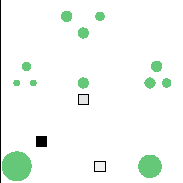
\includegraphics[width=8em]{bilder/instance.pdf}};

% ULF-Instanz:
\node [Box, left of=under-input, text width=14em, node distance=8em] (ULF) 
	{\textbf{ULF-Instanz:} \\ $((\ClientSet\cup\FacilitySet,E),\tilde{c},\phi,d)$ \\
	wobei $\tilde{c}:E \to \IR_{\geq 0}: e \mapsto \frac{2}{u}c(e)$};
\node [Text, left of=ULF, text width=12em, node distance=15em] (ULF-lower-bound) {$\leadsto$ Untere Schranke: $\OPT(\CLR) \geq \OPT(\ULF)$};
\node [Alg, below of=ULF, text width=14em] (ULF-solving) {löse approximativ (mit Greedy)};
\node [Image, left of=ULF-solving, node distance=15em] (ULF-img) {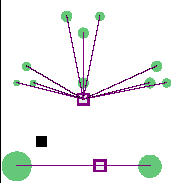
\includegraphics[width=5em]{bilder/ULF.pdf}};

% MST-Instanz:
\node [Box, right of=under-input, text width=14em, node distance=8em] (MST)
	{\textbf{MST-Instanz:} \\ $((\ClientSet\cup\FacilitySet\cup\{r\},E^\prime),c^\prime)$ \\
	$E^\prime := E \cup \{\{r,f\}\mid f\in\FacilitySet\}$ \\
	$c^\prime(f,v) := c(f,v) + \frac{1}{2}\phi(f),$ \\
	$c^\prime(r,f) := 0, c^\prime(v,w):=c(c,w)$};
\node [Text, right of=MST, text width=12em, node distance=15em] (MST-lower-bound) {$\leadsto$ Untere Schranke: $\OPT(\CLR) \geq \OPT(\MST)$};
\node [Alg, below of=MST, text width=14em] (MST-solving) {löse exakt (mit ???)};
\node [Image, right of=MST-solving, node distance=15em] (MST-img) {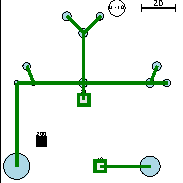
\includegraphics[width=5em]{bilder/MST.pdf}};

% MERGE-Phase:
\node [Text, below of=under-input, node distance=8em] (merge) {\textbf{Merge-Phase:}};

\node [Alg, below of=merge, node distance=1.5em, text width=30em] (m-facilities) {
		\begin{minipage}{30em}\begin{algorithmic}
		\State Eröffne in $\ULF$ oder $\MST$ verwendete Fabriken
		\end{algorithmic}\end{minipage}
	};
\node [Text, left of=m-facilities, node distance=25em, text width=15em] () 
	{beschränkt durch die entsprechenden Eröffnungskosten in $\ULF$ und $\MST$};

% Große Klienten
\node [Alg, below of=m-facilities, node distance=4em] (m-big-clients) {
		\begin{minipage}{30em}\begin{algorithmic}
		\For{Klienten $v$ mit $d(v)\geq u$}
			\State Verbinde $v$ durch $\frac{d(v)}{u}$ Touren mit nächster offener Fabrik
		\EndFor
		\end{algorithmic}\end{minipage}
	};
\node [Image, right of=m-big-clients, node distance=25em] () {
	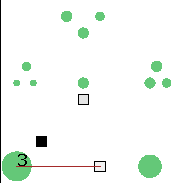
\includegraphics[width=5em]{bilder/largeDemand1.pdf}
	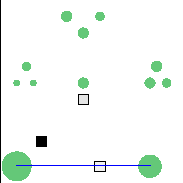
\includegraphics[width=5em]{bilder/largeDemand2.pdf}
};
\node [Text, left of=m-big-clients, node distance=25em, text width=15em] () 
	{beschränkt durch $2\times$ den entsprechenden Verbindungskosten in $\ULF$};

% Kleine Klienten
\node [Alg, below of=m-big-clients, node distance=4em] (m-small-clients) {
		\begin{minipage}{30em}\begin{algorithmic}\algtext*{EndFor}
		\For{Durch $\MST$ eröffnete Fabrik $f$ tue}
		\State Definitionen...
		\EndFor
		\end{algorithmic}\end{minipage}
	};

% Relieve-Schritte
\node [Alg, below of=m-small-clients, node distance=5em] (m-relieve) {
		\begin{minipage}{30em}\begin{algorithmic}\algtext*{For}\algtext*{EndFor}
			\For
			\While{$D_f > 0$}
			\State Finde $v \in S_f$ mit $D_v > u$ und f.a. Kinder $w$ von $v$: $D_w \leq u$
			\State Zerlege $S_v$ in Teilbäume ...
			\EndWhile
			\EndFor
			\end{algorithmic}\end{minipage}
	};
\node [Image, right of=m-relieve, node distance=25em] () {
		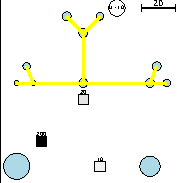
\includegraphics[width=5em]{bilder/relieveTour1.pdf}
		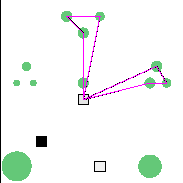
\includegraphics[width=5em]{bilder/relieveTour2.pdf}
		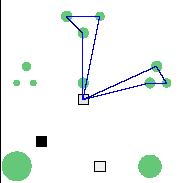
\includegraphics[width=5em]{bilder/relieveTour3.pdf}
	};
\node [Text, left of=m-relieve, node distance=25em, text width=15em] () 
	{Jede Tour ist beschränkt durch $2\times$ die Kantenkosten im $\MST$ und $2\times$ den Verbindungskosten aller Knoten der Tour in $\ULF$};

% Rest
\node [Alg, below of=m-relieve, node distance=5em] (m-remaining) {
		\begin{minipage}{30em}\begin{algorithmic}\algtext*{For}
		\For
		\State Mache Rest
		\EndFor
		\end{algorithmic}\end{minipage}
	};
\node [Image, right of=m-remaining, node distance=25em] () {
	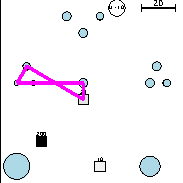
\includegraphics[width=5em]{bilder/remainingTour1.pdf}
	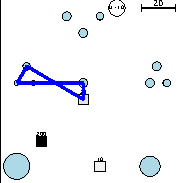
\includegraphics[width=5em]{bilder/remainingTour2.pdf}
};
\node [Text, left of=m-remaining, node distance=25em, text width=15em] () 
	{beschränkt durch $2\times$ den Verbindungskosten in $\MST$};


% AUSGABE:
\node [Box, below of=m-remaining, node distance=3em] (output) {\textbf{Output}};
\node [Image, below of=output] (outpu-img) {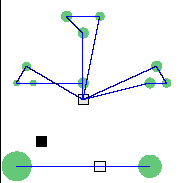
\includegraphics[width=8em]{bilder/output.pdf}};


% PATHS:

\path [arrow] (input.south) -- (ULF.north);    
\path [arrow] (input.south) -- (MST.north); 

\path [arrow] (ULF) -- (ULF-solving.north);
\path [arrow] (MST) -- (MST-solving.north);
\path [arrow] (ULF-solving.south) -- (merge.north);
\path [arrow] (MST-solving.south) -- (merge.north);

\path [line] (m-facilities) -- (m-big-clients);
\path [line] (m-big-clients) -- (m-small-clients);
\path [line] (m-small-clients) -- (m-relieve);
\path [line] (m-relieve) -- (m-remaining);

\path [arrow] (m-remaining.south) -- (output.north);

\end{tikzpicture}

	\end{tiny}
	\caption{Schematische Darstellung des Algorithmus für CLR}
\end{figure}

\subsection{Visualisierung}

\todo[inline]{Beschreibung der Klasse zur Visualisierung}

	

\section{CLR with Hard Facility Capacities (CLRHFC)}

	\subsection{Problemdefinition}

Eine Instanz von \textbf{Capacitated Location Routing with Hard Facility Capacities (CLRHFC)} ist gegeben durch:
\begin{itemize}
	\item eine Instanz $(G=(\ClientSet\cup\FacilitySet,E), c,\phi,d,u)$ von CLR
	\item und zusätzlich Kapazitäten der Fabriken $l: \FacilitySet \to \IR_{\geq 0}$.
\end{itemize}
Zulässige Lösungen sind Lösungen der zugrunde liegenden CLR-Instanz, die zudem die Kapazitätsschranken der Fabriken einhalten.

Das Optimierungsziel weiterhin die Minimierung der Kostenfunktion der CLR-Instanz.

\begin{bem}
	\todo[inline]{Im Unterschied zu harten Kapazitäten gibt es auch die Variante mit weichen Kapazitäten (zumindest für ULF) - vgl. zum Beispiel ...}
\end{bem}

	\subsection{Lösungsansätze}
	
	Zunächst einmal ist klar, dass es nicht genügen wird, nur die Merge-Phase des Algorithmus für $\CLR$ anzupassen. Denn die bereits in der $\ULF$- und der $\MST$-Phase gefällte Entscheidung welche und wie viele Fabriken eröffnet werden, muss offenkundig 

\todo[inline]{Ideen und Probleme für Anpassungen}

	\subsection{Algorithmus}
	
\todo[inline]{Beschreibung des angepassten Algorithmus}

	\subsubsection{Algorithmus 1}
	
	\subsubsection{Algorithmus 2}
	

	\subsection{Implementierungen}
	

	\subsection{Analyse der Algorithmen}
	
	\subsubsection{Theoretische Betrachtungen}

		\todo[inline]{Untere Schranken}
		
		\todo[inline]{Schlechte Beispiele}
		
	\subsubsection{Heuristische Beurteilung}


	\subsection{Ausblick}
	
	\todo[inline]{Was könnte man verbessern? Welche Probleme gibt es dabei?}
	
	

\newpage	
\listoftodos

\newpage
\nocite{*}
\printbibliography		
			
\end{document}